Da die Versuche besonders zeitaufwändig sind, wird darauf verzichtet, alle Messungen von jeder Versuchsgruppe durchzuführen. In dieser Auswertung kann daher nur auf die exakte Versuchsdurchführung der Untersuchung von Gamma-Absorption aus Aufgabenteil II.4 zurück gegriffen werden. Bei den anderen Teilen wird von der Durchführung des Versuchs gemäß der Angaben des Aufgabenblattes ausgegangen.\\

\section{Geiger-Müller-Zählrohr}
\subsection{Einsatzspannung}
Die Spannung des Zählrohrs wird langsam erhöht, gleichzeitig wird die Zählrate gemessen. Der in den Vorbereitungen erläuterte Bereich, in dem die Zählrate gleichmäßig ansteigt, ist in diesem Versuchsaufbau schwierig zu messen. Hier, wie auch in der weiteren Auswertung, wird ein Mittelwert aus den mit \textit{CASSYLAB} aufgenommen Einzelmessungen erzeugt. Die gemessenen Werte enthält Tab \ref{tab:iii_1p1}; eine Auftragung der Zählrate über die Spannung zeigt Abb. \ref{fig:iii_1p1}.

\begin{figure}[ht]
\centering
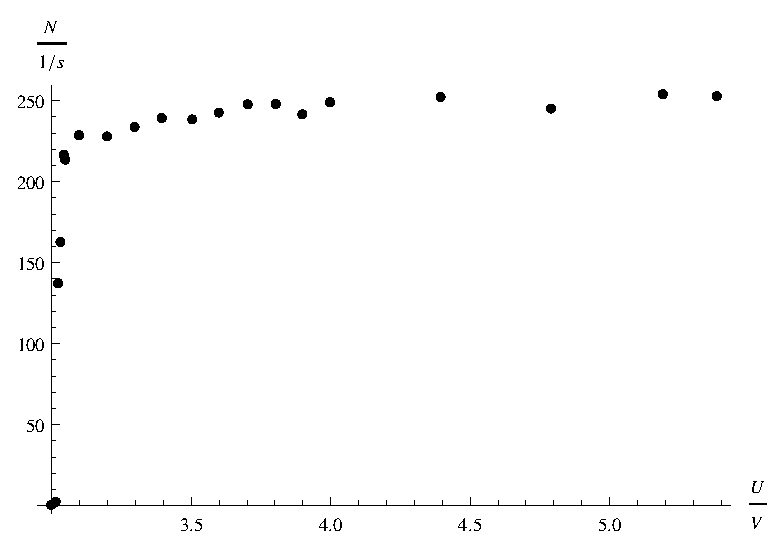
\includegraphics[scale=1.0]{fig/iii_1p1.eps}
\caption{Auftragung der Zählrate über die Einsatzspannung (Aufg 1.1)}
\label{fig:iii_1p1}
\end{figure}

\begin{table}[ht]
\centering
\caption{Messung der Zählrate über die Einsatzspannung (Aufg 1.1)}
\label{tab:iii_1p1}
\begin{tabular}{c|*{8}{*{1}{l}}}
$U$ in $\si{V}$ & $2.997$ & $3.0134$ & $3.0224$ & $3.0308$ & $3.0422$ & $3.0478$ & $3.097$ & $3.1976$ \\ \hline
$N$ in $\si{1/s}$ & $0.4$ & $2.4$ & $137.28$ & $162.88$ & $216.68$ & $213.6$ & $228.76$ & $227.96$\end{tabular}

\begin{tabular}{c|*{8}{*{1}{l}}}
$U$ in $\si{V}$ & $3.2968$ & $3.394$ & $3.5034$ & $3.5982$ & $3.7018$ & $3.8032$ & $3.898$ & $3.9972$ \\ \hline
$N$ in $\si{1/s}$ & $233.8$ & $239.28$ & $238.44$ & $242.72$ & $247.76$ & $247.96$ & $241.64$ & $249.12$\end{tabular}

\begin{tabular}{c|*{4}{*{1}{l}}}
$U$ in $\si{V}$ & $4.3936$ & $4.7898$ & $5.1908$ & $5.3842$ \\ \hline
$N$ in $\si{1/s}$ & $252.4$ & $245.16$ & $254.04$ & $252.84$\end{tabular}

\end{table}

\subsection{Untergrundrate}
Die Untergrundrate der drei Zählrohre wird durch eine Messung der Zählrate über eine Dauer von $\SI{800}{s}$ ohne die Störung durch die radioaktiven Präparate gemessen. Die erhaltenen Untergrundraten enthält Tab. \ref{tab:iii_1p2}.

\begin{table}[ht]
\centering
\caption{Untergrundrate der drei Versuchsaufbauten (Aufg 1.2)}
\label{tab:iii_1p2}
\begin{tabular}{rr}
	\toprule
	Versuch Nr. & $N_0 ~/~ \si{\per\second}$\\
	\midrule
	$1$ & $0{,}40625$\\
	$2$ & $0{,}25000$\\
	$3$ & $0{,}25626$\\
	\bottomrule
\end{tabular}
\end{table}

\subsection{Totzeit}
Wie in den Vorbereitungen erwähnt, wird während der Totzeit nach einer Registrierung kein weiteres Teilchen gemessen. Zunächst soll noch der Zusammenhang der gemessenen, der tatsächlichen Zählrate und der Totzeit ermittelt werden.\\
Die eigentliche Zählrate sei $n$, die gemessene Zählrate $n'$ und die Totzeit $t_\mathrm{tot}$. Nach jedem registrierbaren Teilchen werden damit im Mittel $n \cdot t_\mathrm{tot}$ Teilchen nicht wahrgenommen. Auf jedes gemessene Teilchen kommen daher noch $n \cdot t_\mathrm{tot}$ weitere Teilchen, welche zusammen den tatsächlichen Wert ergeben, also $n = n' + n'nt_\mathrm{tot} = n'(1+nt_\mathrm{tot})$. Durch Umformung erhält man die tatsächliche Zählrate aus der gemessenen:
\begin{equation}
n = \frac{n'}{1-n't_\mathrm{tot}}. \label{eq:iii_1p2_korrektur}
\end{equation}
Dies wird im weiteren Verlauf der Auswertung für die Bestimmung der tatsächlichen Zählrate aus den gemessenen wichtig sein.\\
Aus einer Messung mit zwei Präparaten wie in Aufg. 2, lässt sich die Totzeit ermitteln. Man misst nacheinander die Zählrate mit dem ersten, mit zweiten und zuletzt mit beiden Präparaten. Die tatsächlichen Zählraten $n_1$ und $n_2$ addieren sich, jedoch aufgrund der Totzeit nicht die gemessenen Zählraten $n_1'$ und $n_2'$. Es gilt aber nach obiger Formel \eqref{eq:iii_1p2_korrektur}:
\begin{equation}
\frac{n_1'}{1-n_1't_\mathrm{tot}} + \frac{n_2'}{1-n_2't_\mathrm{tot}} = \frac{n_{1+2}'}{1-n_{1+2}'t_\mathrm{tot}}.
\end{equation}
Man geht in dieser Gleichung zu absoluten Werten über, da im Experiment die absolute Ereigniszahl $N_i'$ in einem festen Zeitintervall $T$ gemessen wurde:
\begin{equation}
\frac{N_1'}{1-N_1'\frac{t_\mathrm{tot}}{T}} + \frac{N_2'}{1-N_2'\frac{t_\mathrm{tot}}{T}} = \frac{N_{1+2}'}{1-N_{1+2}'\frac{t_\mathrm{tot}}{T}}.
\end{equation}
Unter den Zusatzbedingungen $0 < N1$, $0 < N2$, $N1 + N2 < N12$, $T > 0$ und $t_\mathrm{tot} > 0$ löst \textit{Mathematica} dieses Gleichungssystem nach $t_\mathrm{tot}$ mit folgendem Ergebnis auf:
\begin{equation}
t_\mathrm{tot} = \frac{T}{N_{1+2}}\left(1+\sqrt{\frac{(N_{1+2}-N_1)(N_{1+2}-N_2)}{N_1 N_2}}\right).
\end{equation}
Einsetzen der Messwerte der drei Versuchsaufbauten liefert die entsprechenden Totzeiten. Die Ergebnisse enthält Tab. \ref{tab:iii_1p3}.

\begin{table}[ht]
\centering
\caption{Totzeiten der drei Versuchsaufbauten (Aufg 1.3)}
\label{tab:iii_1p3}
\begin{tabular}{c|*{3}{*{1}{l}}}
$\text{Versuch Nr.}$ & $1$ & $2$ & $3$ \\ \hline
$t_{\mathrm{tot}}$ in $\si{ms}$ & $0.0561175$ & $0.133589$ & $0.101034$\end{tabular}

\end{table}

\subsection{Abstandsgesetz}
Zur Verifikation des Abstandsgesetzes wird die Zählrate in Abhängigkeit vom Abstand Präparat-Zählrohr gemessen. Die erhaltenen Werte mitsamt einer Abweichung von $\SI{1}{mm}$ für die Distanzen und einer Standardabweichung der Zählraten enthält Tab. \ref{tab:iii_1p4}. Eine Auftragung dieser zeigt Abb. \ref{fig:iii_1p4_error}. Da hier keine detaillierte Fehlerbetrachtung durchgeführt werden soll, werden auf die Fehler in der logarithmischen Auftragung verzichtet. Eine lineare Regression dieser erfolgt ebenfalls nur auf Basis der Bestwerte. Beide zeigt Abb. \ref{fig:iii_1p4_log}. Also Regressions-Parameter für die logarithmische Anpassung findet man:
\begin{equation}
\log\left(\frac{N}{\si{1/s}}\right) = (-1,45 \pm 0,04) \cdot \log\left(\frac{d}{\si{mm}}\right) + (7,59 \pm 0,13).
\end{equation}
Hierbei wurde der 4. Messpunkt bei notiertem Abstand $d = \SI{30}{mm}$ als Ausreißer eingestuft und nicht in die Regression mit einbezogen. Die Distanzen wurden aus den gemessenen Daten um $\si{5}{mm}$ nach oben korrigiert, da der Abstand der Spitze des Aluminiumstifs zur Stirnfläche etwa $\si{1}{mm}$ und der Abstand von der Stirnfläche zum Präparat $\si{5}{mm}$ betragen. Weiter wurde auf die gemessenen Zählraten die Korrektur aus \eqref{eq:iii_1p2_korrektur} angewandt und anschließend noch die Untergrundzählrate abgezogen (jeweils unter Verwendung der Nullrate und der Totzeit des entsprechenden Versuchsaufbaus).

\begin{table}[p]
\centering
\caption{Messung der Zählrate bei verschiedenen Abständen (Aufg 1.4)}
\label{tab:iii_1p4}
\begin{tabular}{rr}
	\toprule
	$d ~/~ \si{mm}$ & $N ~/~ \si{\per\second}$\\
	\midrule
	$\num{15(2)}$ & $\num{36(5)}$ \\
	$\num{20(2)}$ & $\num{26(6)}$ \\
	$\num{25(2)}$ & $\num{19(3)}$ \\
	$\num{35(2)}$ & $\num{9(3)}$ \\
	$\num{45(2)}$ & $\num{8(2)}$ \\
	$\num{55(2)}$ & $\num{6(3)}$ \\
	$\num{75(2)}$ & $\num{4(2)}$ \\
	$\num{105(2)}$ & $\num{2(1)}$ \\
	\bottomrule
\end{tabular}

\end{table}

\begin{figure}[p]
\centering
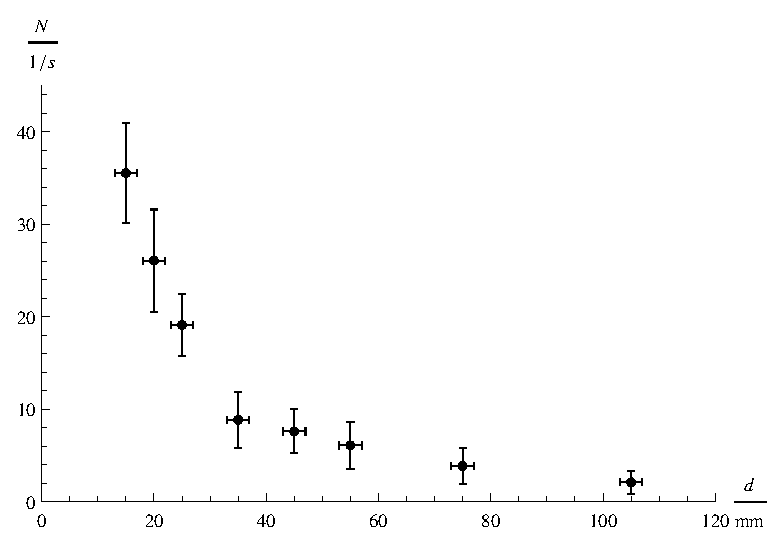
\includegraphics[scale=0.9]{fig/iii_1p4_error.eps}
\caption{Auftragung der Zählrate über die Distanz (Aufg 1.4)}
\label{fig:iii_1p4_error}
\end{figure}

\begin{figure}[p]
\centering
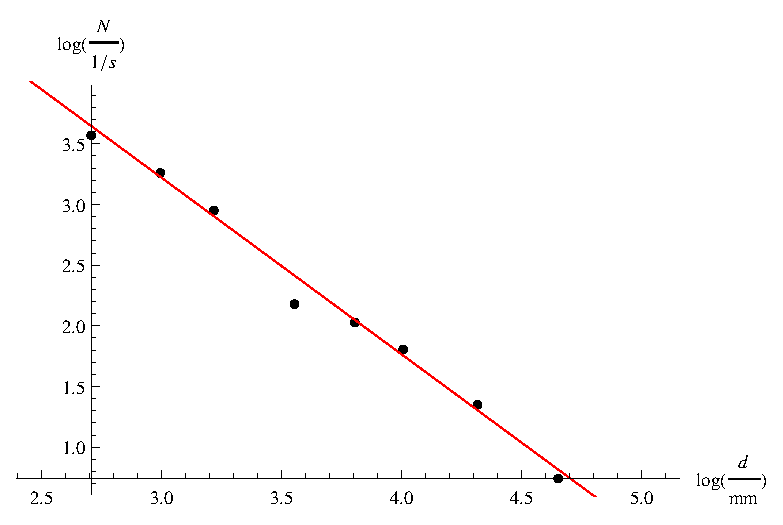
\includegraphics[scale=1.0]{fig/iii_1p4_log.eps}
\caption{Logarithmische Auftragung der Zählrate über die Distanz mit linearer Anpassung (Aufg 1.4)}
\label{fig:iii_1p4_log}
\end{figure}

\section{Absorptionsmessungen}
\subsection{\texorpdfstring{$\upalpha$}{Alpha}-Absorption}
Die Abstände müssen wieder um $\si{8}{mm}$ nach oben korrigiert werden, $\si{7}{mm}$ für den Abstand des Präparats zum Quellrand und $\si{1}{mm}$ für die Eintrittsfensterdicke. Aus den gemessenen Daten wird dann die Zählrate der $\upalpha$-Teilchen ermittelt. Die gemessenen Werte werden wieder gemäß Formel \eqref{eq:iii_1p2_korrektur} korrigiert und anschließend wird die Differenz aus der Messung der Gesamtzählrate und der der $\upgamma$-Teilchen gebildet. Ein Korrektur um die Totzeit ist nicht notwendig, da diese bei der Bildung der Differenz der beiden Messungen bereits entfällt. Anschließend ist noch eine Korrektur des Raumwinkel notwendig, welche gemäß der folgenden Formel vorgenommen wird:
\begin{equation}
\alpha = \alpha' \cdot \frac{2}{1-\cos\arctan(\nicefrac{R}{d})}.\label{eq:iii_2_winkel}
\end{equation}
Hierbei entspricht $R = \si{4,5}{mm}$ dem Radius des Fensters des Zählrohrs und $d$ dem Abstand von Präparat zum Zählrohr. Dieser Zusammenhang soll kurz hergeleitet werden.\\
Die $\upalpha$-Teilchen werden von der punktförmigen Quelle gleichmäßig in alle Raumrichtungen abgestrahlt. Sei $\alpha(x)$ der Teil der $\upalpha$-Teilchen, der nach dem Durchdringen einer Luftschicht der Dicke $x$ noch vorhanden ist. Dann ist der Anteil der $\upalpha$-Teilchen der punktförmigen Quelle im Abstand $r$ im Raumwinkelstück $\omega$:
\begin{equation}
\alpha' = \alpha(r) \cdot \frac{\omega}{4 \uppi}.\label{eq:iii_2_abh}
\end{equation}
Gemessen wird die Zählrate am Zählrohr, $\alpha'$. Gesucht ist jedoch die Abhängigkeit der Zahl der $\upalpha$-Teilchen von der zurück gelegten Distanz $\alpha(x)$. Es folgt somit:
\begin{equation}
\alpha(d) = \alpha' \cdot \frac{4\uppi}{\omega}.
\end{equation}
Gefragt ist jetzt also nur noch das Raumwinkelstück $\omega$ in Abhängigkeit vom Abstand $d$ von Präparat zum Zählrohr und vom Radius $R$ des Zählrohrfensters.\\
Dazu führt man folgende Rechnung durch: Man legt die Quelle in den Ursprung und untersucht den Raumwinkel einer Kreisscheibe des Radius $R$ im Abstand $d$ von diesem Punkt aus. Man wähle die Polarkoordinaten zur Integration mit der z-Achse in Richtung des Mittelpunktes der Scheibe und findet so den maximalen Öffnungswinkel $\Theta = \arctan(\nicefrac{R}{d})$. Die Integration liefert dann:
\begin{align}
\omega &= \int \frac{\hat{n}\cdot d\vec{a}}{\rho^2} = \int_0^{2 \pi} d\phi \left( \int_0^{\arctan\left(\frac{R}{d}\right)} d\Theta \sin\left(\Theta\right) \right)\nonumber\\
&= 2\pi \cdot \left[ -\cos(\Theta) \right]_{\theta=0}^{\theta=\arctan\left(\frac{R}{d}\right)}\nonumber\\
&= 2\pi \cdot (1-\cos(\arctan(\nicefrac{R}{d})))
\end{align}
Mit Gl. \eqref{eq:iii_2_abh} folgt so die Relation aus Gl. \eqref{eq:iii_2_winkel}. Mithilfe sämtlicher Korrekturen erhält man nun den Bestand der $\upalpha$-Teilchen in Abhängigkeit von der durchdrungenen Materie. Die berechneten Werte enthält Tab. \ref{tab:iii_2}. Eine Auftragung ohne Raumwinkel-Korrektur befindet sich in Abb. \ref{fig:iii_2_plota}; eine Auftragung mit Raumwinkel-Korrektur und einer linearen Regression der ersten Messpunkte (jener im annähernd linearen Bereich) findet sich in Abb. \ref{fig:iii_2_plotb}. Die Regression wurde aus folgenden Gründen so gewählt.

\begin{figure}[ht]
\centering
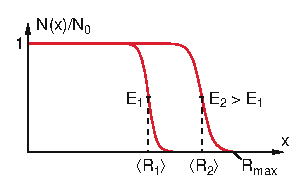
\includegraphics[scale=1.5]{fig/iii_2_dem.eps}
\caption{Abnahme der $\upalpha$-Teilchen $N(x)$ über die durchdrungene Materie $x$; Quelle: \cite[S. 90]{Dem10}}
\label{fig:iii_2_dem}
\end{figure}

Abb. \ref{fig:iii_2_dem} zeigt die voraus gesagte Abnahme der $\upalpha$-Teilchen beim Durchdringen der Materie. Die Teilchenzahl bleibt zunächst konstant, nimmt dann rasch ab und bleibt dann konstant bei 0. Die entsprechend definierte mittlere Reichweite ist in dieser Abb. ebenfalls  eingezeichnet. Den genannten Kurvenverlauf findet man auch bei der Auftragung der hier gemessenen Werte (s. Abb. \ref{fig:iii_2_plotb}). Man fittet an die Werte im nicht konstanten Bereich eine Gerade an und sucht den Punkt, an dem sie auf die Hälfte des Wertes abgefallen ist, der für kleine Abstände vorliegt (verwende hier 11. Messpunkt bei ungefähr $\si{4}{mm}$), und findet so die mittlere Reichweite $\anglemean R$. Als Geradengleichung ergibt sich:
\begin{equation}
N(x) = -(890 \pm 100)\frac{x}{\si{cm}} + (27330 \pm 750),
\end{equation}
welche ebenfalls in genannter Abb. \ref{fig:iii_2_plotb} eingezeichnet ist. Die mittlere Reichweite berechnet sich so unter der Verwendung der Bestwerte zu:
\begin{equation}
\anglemean R = \SI{15,8}{cm}.
\end{equation}
Die letzten drei Messwerte wurden bei der Regression vernachlässigt, da sie aufgrund der Hintergrundstrahlung zu starke statistische Abweichungen aufweisen.

\begin{figure}[ht]
\centering
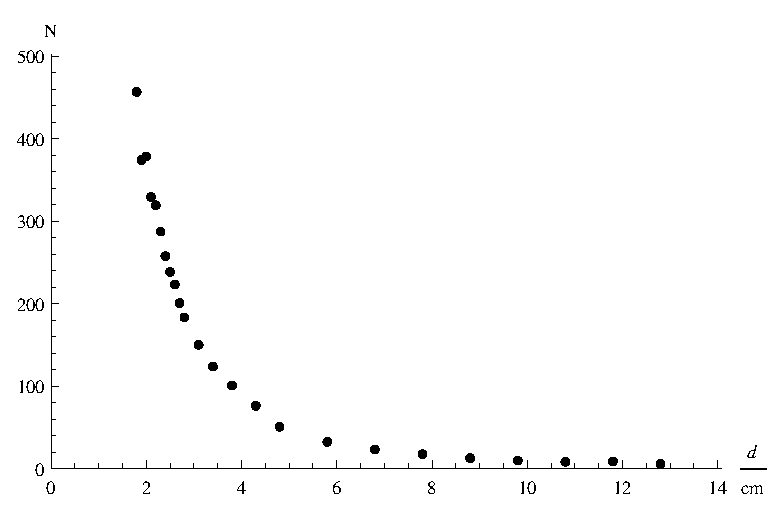
\includegraphics[scale=1.0]{fig/iii_2_plota.eps}
\caption{Zählrate der $\upalpha$-Teilchen am Zählrohr (Aufg. 2)}
\label{fig:iii_2_plota}
\end{figure}

\begin{figure}[ht]
\centering
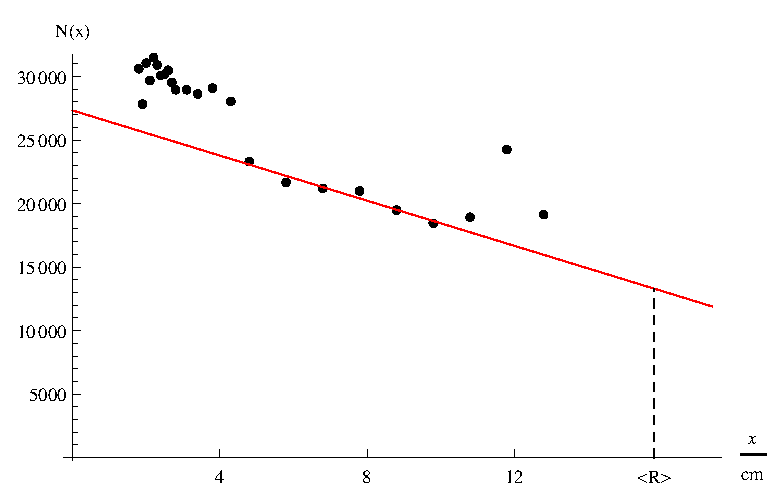
\includegraphics[scale=1.0]{fig/iii_2_plotb.eps}
\caption{Abnahme der $\upalpha$-Teilchen bei Durchgang durch die Materie der Strecke $x$ mit Raumwinkel-Korrektur und lin. Regression der ersten Messpunkte (annähernd lin. Bereich) (Aufg. 2)}
\label{fig:iii_2_plotb}
\end{figure}

\begin{table}[ht]
\centering
\caption{Abnahme der $\upalpha$-Teilchen bei Durchgang durch die Materie mit ($\alpha$) und ohne ($\alpha'$) Raumwinkel-Korrektur (Aufg. 2)}
\label{tab:iii_2}
\begin{tabular}{c|*{8}{*{1}{l}}}
$d$ in ${\si{cm}}$ & $1.8$ & $1.9$ & $2.$ & $2.1$ & $2.2$ & $2.3$ & $2.4$ & $2.5$ \\ \hline
$\alpha'$ & $456.876$ & $374.393$ & $378.652$ & $329.51$ & $319.526$ & $287.534$ & $257.715$ & $238.58$ \\ \hline
$\alpha$ & $30603.8$ & $27815.5$ & $31049.5$ & $29688.9$ & $31503.6$ & $30905.5$ & $30093.1$ & $30168.2$\end{tabular}

\begin{tabular}{c|*{8}{*{1}{l}}}
$d$ in ${\si{cm}}$ & $2.6$ & $2.7$ & $2.8$ & $3.1$ & $3.4$ & $3.8$ & $4.3$ & $4.8$ \\ \hline
$\alpha'$ & $223.334$ & $200.804$ & $183.421$ & $150.155$ & $123.726$ & $100.909$ & $76.1512$ & $50.8601$ \\ \hline
$\alpha$ & $30490.4$ & $29516.8$ & $28954.4$ & $28953.1$ & $28622.9$ & $29085.$ & $28041.3$ & $23299.5$\end{tabular}

\begin{tabular}{c|*{8}{*{1}{l}}}
$d$ in ${\si{cm}}$ & $5.8$ & $6.8$ & $7.8$ & $8.8$ & $9.8$ & $10.8$ & $11.8$ & $12.8$ \\ \hline
$\alpha'$ & $32.4645$ & $23.1334$ & $17.4194$ & $12.7102$ & $9.70605$ & $8.20414$ & $8.80464$ & $5.90235$ \\ \hline
$\alpha$ & $21669.8$ & $21199.$ & $20986.4$ & $19480.6$ & $18442.3$ & $18927.$ & $24242.9$ & $19119.8$\end{tabular}

\end{table}

\subsection{\texorpdfstring{$\upbeta$}{Beta}-Absorption}
Die gemessenen Werte werden natürlich zunächst wieder unter Berücksichtigung der Totzeit mittels Gl. \eqref{eq:iii_1p2_korrektur} und der Nullrate korrigiert. Die Werte enthält Tab. \ref{tab:iii_3}.

\begin{table}[ht]
\centering
\caption{Zahl der $\upbeta$-Teilchen nach Durchgang der Dicke $d$ (Aufg. 3)}
\label{tab:iii_3}
\begin{tabular}{c|*{8}{*{1}{l}}}
$x$ in $\si{\micro\meter}$ & $18.$ & $22.$ & $24.5$ & $34.8$ & $37.$ & $62.$ & $112.$ & $212.$ \\ \hline
$N$ in $\si{1/s}$ & $101.104$ & $100.144$ & $100.408$ & $95.825$ & $93.5614$ & $85.1875$ & $71.3028$ & $54.1492$\end{tabular}

\begin{tabular}{c|*{7}{*{1}{l}}}
$x$ in $\si{\micro\meter}$ & $322.$ & $537.$ & $992.$ & $1472.$ & $2002.$ & $3012.$ & $4012.$ \\ \hline
$N$ in $\si{1/s}$ & $48.1106$ & $34.8517$ & $20.9125$ & $10.865$ & $5.29$ & $0.9225$ & $0.3875$\end{tabular}

\end{table}

\begin{figure}[ht]
\centering
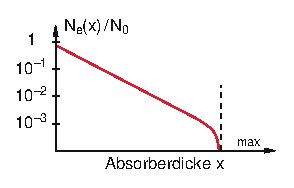
\includegraphics[scale=1.5]{fig/iii_3_dem.eps}
\caption{Abnahme der $\upbeta$-Teilchen $N(x)$ über die durchdrungene Materie $x$; Quelle: \cite[S. 92]{Dem10}}
\label{fig:iii_3_dem}
\end{figure}

Obige Abb. \ref{fig:iii_3_dem} zeigt den vorausgesagten Verlauf. Es wird die Teilchenzahl logarithmisch gegen den Abstand $x$ aufgetragen. Dabei ergibt sich für geringe Abstände ein linearer Abfall und ab einem bestimmten Punkt eine noch stärkere Abnahme. Die Teilchenzahl sinkt also für eine kurze Zeit exponentiell und dann nochmals deutlich schneller auf 0 ab, ihr Logarithmus dann also auf $-\infty$. Letzter Bereich ist in diesem Experiment schwer beobachtbar, gut ablesbar ist nur der lineare Bereich. Genau den letzten Teil der schnellen Abnahme ist aber bedeutend für die Reichweite der Teilchen. Es wird also eine lineare Anpassung an den ersten Bereich erstellt und der Punkt gesucht, an dem der Einbruch statt findet, was in etwa der maximalen Reichweite entspricht. In Abb. \ref{fig:iii_3_dem} tritt das etwa bei $\log(\nicefrac{N}{N_0}) = 10^{-3}$ ein. In diesem Versuch finden sich zwei Messpunkte bei ca. $\SI{3000}{\micro\meter}$ und $\SI{4000}{\micro\meter}$, welche beide bereits im Untergrundbereich liegen. Erster ist nur noch minimal größer als Zählrate 0 und zweiter liegt sogar im negativen Bereich. Man geht daher davon aus, dass bei Messpunkt $x=\SI{3000}{\micro\meter}$ der Einbruch stattfindet. Genauer handelt es sich hierbei um den Einbruch der Zerfalls-Strahlung höherer Reichweite. Dass in diesem Versuch zwei Zerfälle zu beobachten sind, lässt sich auch anhand der logarithmischen Auftragung der Messwerte erkennen. Dort gibt es bereits bei kleinen $x$ einen linearen Bereich mit noch geringerer Steigung. Das Verfahren lautet insgesamt also viel folgt:\\
An den linearen Bereich von $\SI{500}{\micro\meter}$ bis $\SI{2000}{\micro\meter}$ wird eine lineare Funktion angefittet und der Schnittpunkt mit dem logarithmischen Wert des Messpunktes bei $x=\SI{3000}{\micro\meter}$ gesucht. Dies entspricht der maximalen Reichweite der Teilchen hoher Reichweite. Die Teilchen niedriger Reichweite sind bereits früher abgefallen und stören diese Untersuchung nicht mehr. Um nun dieses Verfahren auch auf die Teilchen niedriger Reichweite anwenden zu können, werden diese um die nun bekannte Zählrate der höherenergetischen Strahlung im Bereich $x < \SI{500}{\micro\meter}$ subtrahiert, da sich diese Werte als Überlagerung beider Zerfälle ergeben. Dies liefert als maximale Reichweite für den höherenergetischen $\element{Y}{39}{90}$-Zerfall:
\begin{equation}
R_\mathrm{max} (\element{Y}{39}{90} \xrightarrow{\upbeta^-} \element{Zr}{40}{90}) \approx \SI{3000}{\micro\meter},
\end{equation}
und für den niederenergetischen $\element{Sr}{38}{90}$-Zerfall:
\begin{equation}
R_\mathrm{max} (\element{Sr}{38}{90} \xrightarrow{\upbeta^-} \element{Y}{39}{90}) \approx \SI{168}{\micro\meter}.
\end{equation}
Die linearen Regressionen ergeben die Zusammenhänge
\begin{equation}
\log\left(\frac{N}{\si{1/s}}\right) = (-1,34 \pm 0,04) \cdot 10^{-3} \cdot \log\left(\frac{d}{\si{mm}}\right) + (4,30 \pm 0,07).
\end{equation}
für die höherenergetische Strahlung und
\begin{equation}
\log\left(\frac{N}{\si{1/s}}\right) = (-20,7 \pm 1,5) \cdot 10^{-3} \cdot \log\left(\frac{d}{\si{mm}}\right) + (3,75 \pm 0,05).
\end{equation}
für niederenergetische Strahlung. Mit der Dichte des Absorbermaterials $\rho=\SI{2,71}{\gram\centi\meter^{-3}}$ folgt so der Massenabsorptionskoeffizient für die höherenergetische Strahlung:
\begin{equation}
\kappa = \frac{(-1,34 \pm 0,04) \cdot 10^{-3}}{\SI{2,71}{\gram\centi\meter^{-3}}} \approx (0,494 \pm 0,015) \times 10^{-6} \si{m^3/kg},
\end{equation}
und für die niederenergetische Strahlung:
\begin{equation}
\kappa = \frac{((-20,7 \pm 1,5) \cdot 10^{-3}}{\SI{2,71}{\gram\centi\meter^{-3}}} \approx (7,6 \pm 0,5) \times 10^{-6} \si{m^3/kg}.
\end{equation}
Mithilfe der auf dem Aufgabenblatt gegebenen Flammersfeld-Beziehung folgt außerdem die Grenzenergie des höherenergetischen Zerfalls,
\begin{equation}
W_\mathrm{Gr} = \SI{1760}{keV},
\end{equation}
und die des niederenergetischen,
\begin{equation}
W_\mathrm{Gr} = \SI{211}{keV},
\end{equation}
was in etwa in der Größenordnung der Literatur-Werte liegt ($\SI{2284}{keV}$, bzw. $\SI{540}{keV}$).

\begin{figure}[ht]
\centering
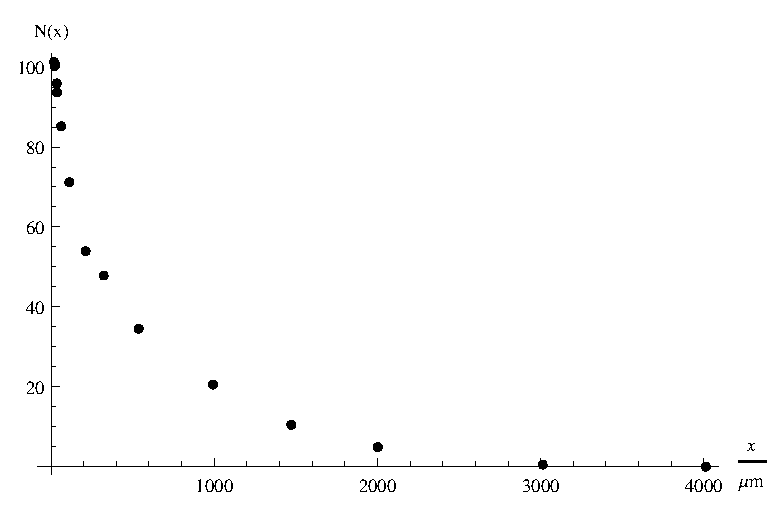
\includegraphics[scale=1.0]{fig/iii_3_plota.eps}
\caption{Auftragung der Zählrate $N(x)$ über die Absorberdicke $x$ (Aufg. 3)}
\label{fig:iii_3_plota}
\end{figure}

\begin{figure}[p]
\centering
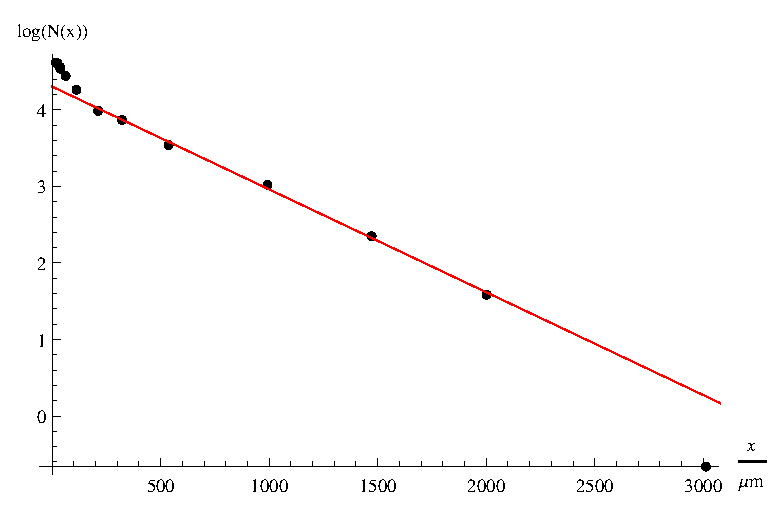
\includegraphics[scale=1.0]{fig/iii_3_plotb.eps}
\caption{Logarithmische Auftragung der Zählrate $\log(N(x))$ über die Absorberdicke $x$ mit lin. Regression des Bereiches großer $x$ (Aufg. 3)}
\label{fig:iii_3_plotb}
\end{figure}

\begin{figure}[p]
\centering
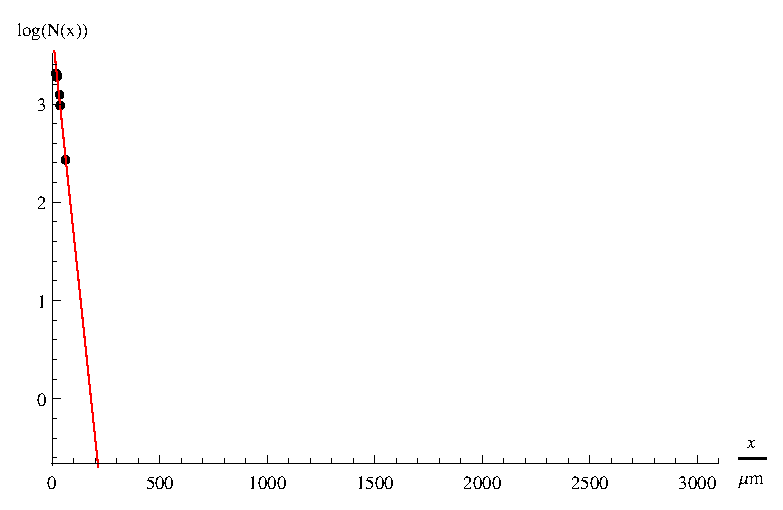
\includegraphics[scale=1.0]{fig/iii_3_plotc.eps}
\caption{Logarithmische Au
ftragung der Zählrate der Teilchen geringer Reichweite $\log(N(x))$ über die Absorberdicke $x$ mit lin. Regression(Aufg. 3)}
\label{fig:iii_3_plotc}
\end{figure}

Zuletzt bleibt noch die Frage danach, in welchem Verhältnis die beiden Zerfallsarten vorliegen werden. Eine Rechnung mit üblichen Modellen der physikalischen Chemie befindet sich in Anhang A.
Die Rechnung ergibt, dass das Verhältnis von Yttrium-Zerfall zu Strontium-Zerfall ungefähr 1 ist, genauer $\frac{k_\mathrm{Y}}{k_\mathrm{Y} - k_\mathrm{Sr}}$. Der Rechnung entnimmt man weiter, dass sich das System diesem Zustand über die Zeit gemäß eines exponentiellen, beschränkten Wachstums annähert.

\subsection{\texorpdfstring{$\upgamma$}{Gamma}-Absorption}
\subsubsection{Blei-Absorption von Co60-Strahlung}
Die gemessenen Werte werden wieder gemäß Gl. \eqref{eq:iii_1p2_korrektur} sowie um die Nullrate korrigiert und anschließend doppeltlogarithmisch aufgetragen. Die berechneten Werte enthält Tab. \ref{tab:iii_4p1}; die Auftragung mit linearer Regression zeigt Abb. \ref{fig:iii_4p1}. Die Regression ergibt als Fit-Parameter:
\begin{equation}
\log\left(\frac{N}{\si{1/s}}\right) = (-0,35 \pm 0,06) \cdot \log\left(\frac{d}{\si{mm}}\right) + (2,71 \pm 0,13).
\end{equation}

\begin{table}[p]
\centering
\caption{Korrigierte Zählraten bei verschiedenen Absorberdicken (Aufg. 4.1)}
\label{tab:iii_4p1}
\begin{tabular}{rr}
	\toprule
	$d ~/~ \si{\milli\meter}$ & $N ~/~ \si{\per\second}$\\
	\midrule
	$\num{1}$ & $\num{12.597}$ \\
	$\num{2}$ & $\num{12.009}$ \\
	$\num{5}$ & $\num{10.2855}$ \\
	$\num{10}$ & $\num{7.80263}$ \\
	$\num{15}$ & $\num{6.30286}$ \\
	$\num{20}$ & $\num{4.76834}$ \\
	$\num{25}$ & $\num{3.84654}$ \\
	\bottomrule
\end{tabular}

\end{table}

\begin{figure}[p]
\centering
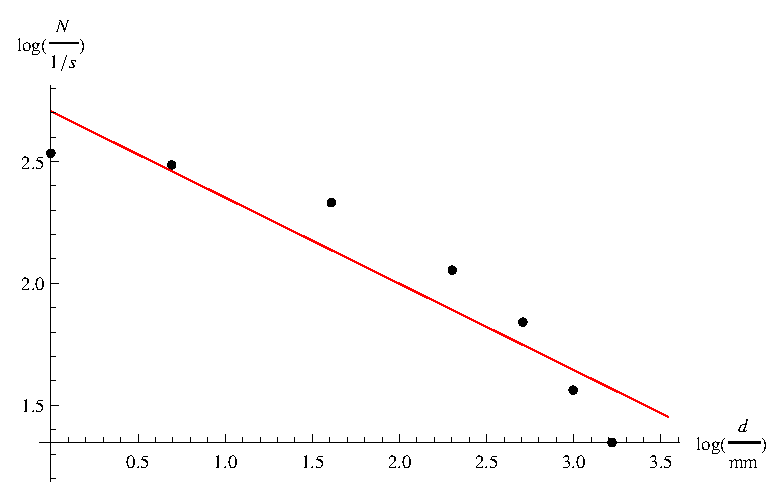
\includegraphics[scale=1.0]{fig/iii_4p1.eps}
\caption{Doppeltlogarithmische Auftragung der korrigierten Werte mit linearer Regression (Aufg. 4.1)}
\label{fig:iii_4p1}
\end{figure}

\subsubsection{Blei-Absorption von Cs137-Strahlung}
Das Verfahren ist analog zu dem aus Aufgabenteil 4.1. Die berechneten Werte enthält Tab. \ref{tab:iii_4p2}; die Auftragung mit linearer Regression zeigt Abb. \ref{fig:iii_4p2}. Die Regression ergibt als Fit-Parameter:
\begin{equation}
\log\left(\frac{N}{\si{1/s}}\right) = (-0,73 \pm 0,17) \cdot \log\left(\frac{d}{\si{mm}}\right) + (3,0 \pm 0,4).
\end{equation}

\begin{table}[p]
\centering
\caption{Korrigierte Zählraten bei verschiedenen Absorberdicken (Aufg. 4.2)}
\label{tab:iii_4p2}
\begin{tabular}{c|*{7}{*{1}{l}}}
$d$ in ${\si{mm}}$ & $1$ & $2$ & $5$ & $10$ & $15$ & $20$ & $25$ \\ \hline
$N$ in ${\si{1/s}}$ & $12.4932$ & $11.2221$ & $11.0592$ & $5.26505$ & $3.27983$ & $1.85586$ & $0.954194$\end{tabular}

\end{table}

\begin{figure}[p]
\centering
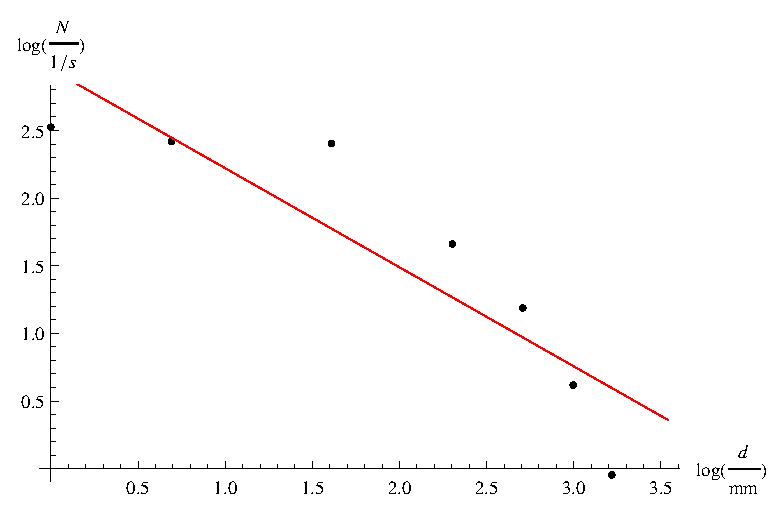
\includegraphics[scale=1.0]{fig/iii_4p2.eps}
\caption{Doppeltlogarithmische Auftragung der korrigierten Werte mit linearer Regression (Aufg. 4.2)}
\label{fig:iii_4p2}
\end{figure}

\subsubsection{Absorption verschiedener Materialien}
Da im Versuch die absolute Strahlung ohne Absorber nicht gemessen wurde, muss sich hier auf absolute Angaben der Strahlung beschränkt werden. Die gemessenen und korrigierten Werte enthält Tab. \ref{tab:iii_4p3}. Eine Auftragung über die Dichte zeigt Abb. \ref{fig:iii_4p3}.

\begin{table}[p]
\centering
\caption{Strahlintensität bei verschiedenen Abschirmmaterialien (Aufg. 4.3)}
\label{tab:iii_4p3}
\begin{tabular}{c|*{4}{*{1}{l}}}
$\text{Material}$ & $\text{Messing}$ & $\text{Eisen}$ & $\text{Beton}$ & $\text{Aluminium}$ \\ \hline
$\rho$ in ${\nicefrac{g}{cm^3}}$ & $8.4$ & $7.8$ & $2.14$ & $2.71$ \\ \hline
$N$ in ${\nicefrac{1}{s}}$ & $5.99962$ & $6.73673$ & $10.0321$ & $10.4675$\end{tabular}

\begin{tabular}{c|*{3}{*{1}{l}}}
$\text{Material}$ & $\text{Trovidur}$ & $\text{Plexiglas}$ & $\text{Hartholz}$ \\ \hline
$\rho$ in ${\si{g/cm^3}}$ & $1.38$ & $1.18$ & $0.68$ \\ \hline
$N$ in ${\si{1/s}}$ & $11.6378$ & $12.1929$ & $12.434$\end{tabular}

\end{table}

\begin{figure}[p]
\centering
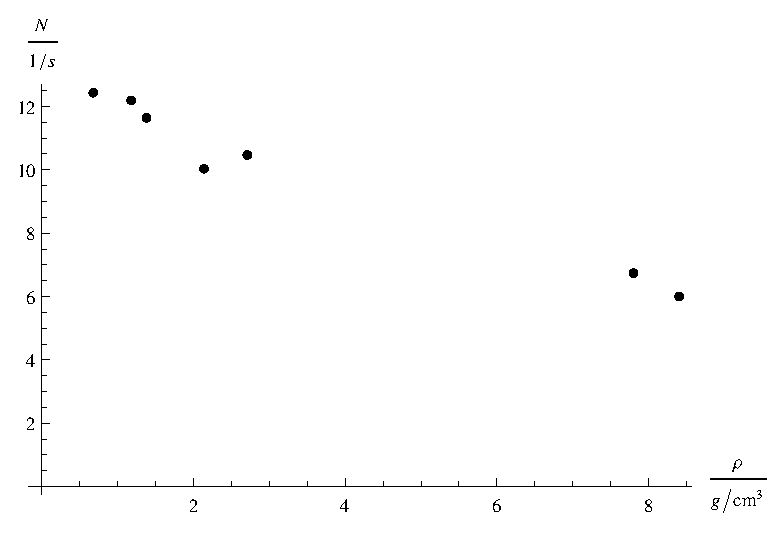
\includegraphics[scale=1.0]{fig/iii_4p3.eps}
\caption{Auftragung der gemessenen Strahlintensitäten über die Dichten der Abschirmmaterialien (Aufg. 4.3)}
\label{fig:iii_4p3}
\end{figure}

\begin{table}[ht]
	\begin{center}
		\rowcolors{3}{gray!10}{white}
		\caption{Werte für jede freie Schwingung, zugeordnet zur Dämpfung $l$ durch die Wirbelstrombremse:
		Periodendauer $T$, Eigenfrequenz $\omega_\text{e}$, logarithmisches Dekrement $\Lambda$, Dämpfungskonstante $\beta$ und
		die ungedämpfte Eigenfrequenz $\omega_0$.}
		\begin{tabular}{rrrrrr}
			\toprule
			$l ~/~ \si{\milli\meter}$ & $T ~/~ \si\second$ & $\omega_{\mathrm{e}} ~/~ \si{\milli\Hz}$ & $\Lambda$ & $\beta ~/~ \si{\per\s}$ & $\omega_0 ~/~ \si{\milli\Hz}$\\
			\midrule
			$\num{0}$ & $\num{3.026} \pm \num{0.013}$ & $\num{330.5} \pm \num{1.5}$ & $\num{0.081} \pm \num{0.007}$ & $\num{0.027} \pm \num{0.003}$ & $\num{330.5} \pm \num{1.5}$\\
			$\num{4}$ & $\num{2.95} \pm \num{0.03}$   & $\num{339} \pm \num{3}$     & $\num{0.33} \pm \num{0.03}$   & $\num{0.111} \pm \num{0.009}$ & $\num{340} \pm \num{3}$\\
			$\num{6}$ & $\num{2.91} \pm \num{0.03}$   & $\num{344} \pm \num{4}$     & $\num{0.71} \pm \num{0.08}$   & $\num{0.25} \pm \num{0.03}$   & $\num{346} \pm \num{4}$\\
			$\num{8}$ & $\num{2.92} \pm \num{0.08}$   & $\num{343} \pm \num{9}$     & $\num{1.07} \pm \num{0.08}$   & $\num{0.37} \pm \num{0.03}$   & $\num{348} \pm \num{9}$\\
			\bottomrule
		\end{tabular}
		\label{tab:frei}
	\end{center}
\end{table}